% Chapter 1

\chapter{Exploratory Data Analysis (EDA)} % Main chapter title

\label{Chapter1} % For referencing the chapter elsewhere, use \ref{Chapter1} 

\lhead{\emph{Exploratory Data Analysis (EDA)}} % This is for the header on each page - perhaps a shortened title

%----------------------------------------------------------------------------------------

{EDA: Making use of various Pandas functions, I conducted some initial analysis of our dataset}

% OLD TABLE 

\begin{table}[htbp]
\centering
\begin{tabular}{|>{\columncolor[HTML]{EFEFEF}}l|l|}
\hline
Invoice ID & 750-67-8428   \\ \hline
Branch & A   \\ \hline
City & Yangon   \\ \hline
Customer type & Member   \\ \hline
Gender & Female   \\ \hline
Product line & Health and beauty   \\ \hline
Unit price & 74.69   \\ \hline
Quantity & 7   \\ \hline
Tax 5\% & 26.1415   \\ \hline
Total & 548.9715  \\ \hline
Payment & Ewallet  \\ \hline
Date & 1/5/2019  \\ \hline
Time & 13:08  \\ \hline
cogs & 522.83  \\ \hline
gross income & 26.1415  \\ \hline
Rating & 9.1  \\ \hline
\end{tabular}
% \caption{Example two-column table with colored first column}
% \label{tab:example_table_two_columns}
\end{table}





%----------------------------------------------------------------------------------------


\newpage 

\begin{table}[htbp]
    \centering
    {Using Pandas’ describe function, I was able to gain insight into the numerical features}
    \newline
    \newline
    \renewcommand{\arraystretch}{2} % Adjust the vertical spacing between rows
    \resizebox{\textwidth}{!} & \cellcolor[HTML]{007000}\textcolor{white}{Total} & \cellcolor[HTML]{007000}\textcolor{white}{cogs} & \multirow{2}{*}{\cellcolor[HTML]{007000}\textcolor{white}{\shortstack{gross margin\\ percentage}}} & \cellcolor[HTML]{007000}\textcolor{white}{gross income} & \cellcolor[HTML]{007000}\textcolor{white}{Rating} \\ \hline
        count   & 1000.0000   & 1000.0000   & 1000.0000   & 1000.0000   & 1000.0000   & 1000.0000   & 1000.0000   & 1000.0000   \\ \hline
        \rowcolor[HTML]{DDFFDD} 
        mean  & 55.672130  & 5.510000  & 15.379369  & 322.966749  & 307.58738  & 4.761905  & 15.379369  & 6.97270  \\ \hline
        std  & 26.494628  & 2.923431  & 11.708825  & 245.885335  & 234.17651  & 0.000000  & 11.708825  & 1.71858\\ \hline
        \rowcolor[HTML]{DDFFDD} 
        min  & 10.080000  & 1.000000  & 0.508500  & 10.678500  & 10.17000  & 4.761905  & 0.508500  & 4.00000  \\ \hline
        25\%  & 32.875000  & 3.000000  & 5.924875  & 124.422375  & 118.49750  & 4.761905  & 5.924875  & 5.50000  \\ \hline
        \rowcolor[HTML]{DDFFDD} 
        50\%  & 55.230000  & 5.000000  & 12.088000  & 253.848000  & 241.76000  & 4.761905  & 12.088000  & 7.00000  \\ \hline
        75\%  & 77.935000  & 8.000000  & 22.445250  & 471.350250  & 448.90500  & 4.761905  & 22.445250  & 8.50000  \\ \hline
        \rowcolor[HTML]{DDFFDD} 
        max  & 99.960000  & 10.000000  & 49.650000  & 1042.650000  & 993.00000  & 4.761905  & 49.650000  & 10.00000  \\ \hline
    \end{tabular}%
    }
%    \caption{}
%    \label{tab:example_table_9_by_9}
\end{table}


% \section{Observation:}
On average, customers spend approximately \$322.97 per transaction, with a standard deviation of \$245.89, indicating significant variability. The constant gross margin percentage of 4.76\% suggests a consistent profit margin, while customer ratings, averaging 6.97 with a standard deviation of 1.72, reflect overall satisfaction. 
% -------------------------------------------------------------------------------
{Distribution of numerical columns}
The visualizations below are to help us understand the distribution of some numerical columns. The x-axis of each histogram represents the range of values, and the y-axis represents the frequency (count) of data points within each range. The number of bins (20 in this case) determines the granularity of the distribution. The feature ‘Unit Price’ seems to be quite heavily and evenly distributed. In contrast, ‘Quantity’ sparsely populates its chart. The ‘Total’ and ‘Tax’ columns both show a central tendency towards higher values.


\begin{figure}[h]
    \centering
    \begin{subfigure}[b]{0.2\textwidth}
        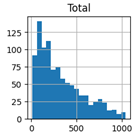
\includegraphics[width=\textwidth]{Chapters/ch1/n_dist_1.png}
        % \caption{Image A}
        % \label{fig:sub1}
    \end{subfigure}
    \hspace{0.05\textwidth} % Adjust the spacing between images
    \begin{subfigure}[b]{0.2\textwidth}
        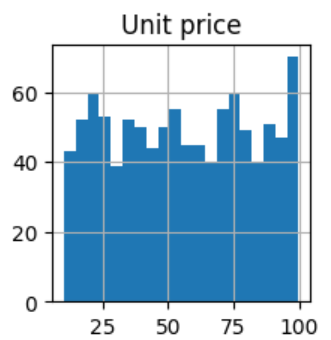
\includegraphics[width=\textwidth]{Chapters/ch1/unit-price.png}
        % \caption{Image B}
        % \label{fig:sub2}
    \end{subfigure}
    \hspace{0.05\textwidth} % Adjust the spacing between images
    \begin{subfigure}[b]{0.2\textwidth}
        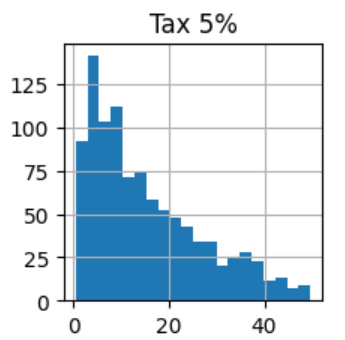
\includegraphics[width=\textwidth]{Chapters/ch1/tax.png}
        % \caption{Image C}
        % \label{fig:sub3}
    \end{subfigure}
    \hspace{0.05\textwidth} % Adjust the spacing between images
    \begin{subfigure}[b]{0.2\textwidth}
        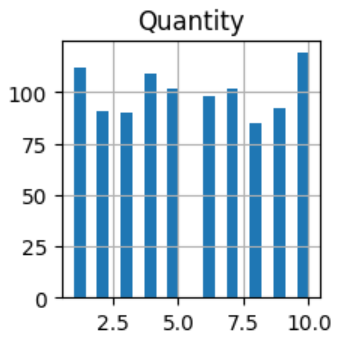
\includegraphics[width=\textwidth]{Chapters/ch1/quantity.png}
        % \caption{Image D}
        % \label{fig:sub4}
    \end{subfigure}
    % \caption{Four images in a row}
    % \label{fig:allimages}
\end{figure}




% If you are new to \LaTeX{}, there is a very good eBook -- freely available online as a PDF file -- called, ``The Not So Short Introduction to \LaTeX{}''. The book's title is typically shortened to just ``lshort''. You can download the latest version (as it is occasionally updated) from here:\\
% \href{http://www.ctan.org/tex-archive/info/lshort/english/lshort.pdf}{\texttt{http://www.ctan.org/tex-archive/info/lshort/english/lshort.pdf}}

% It is also available in several other languages. Find yours from the list on this page:\\
% \href{http://www.ctan.org/tex-archive/info/lshort/}{\texttt{http://www.ctan.org/tex-archive/info/lshort/}}

% It is recommended to take a little time out to learn how to use \LaTeX{} by creating several, small `test' documents. Making the effort now means you're not stuck learning the system when what you \emph{really} need to be doing is writing your thesis.

% \subsection{A Short Math Guide for \LaTeX{}}

% If you are writing a technical or mathematical thesis, then you may want to read the document by the AMS (American Mathematical Society) called, ``A Short Math Guide for \LaTeX{}''. It can be found online here:\\
% \href{http://www.ams.org/tex/amslatex.html}{\texttt{http://www.ams.org/tex/amslatex.html}}\\
% under the ``Additional Documentation'' section towards the bottom of the page.

% \subsection{Common \LaTeX{} Math Symbols}
% There are a multitude of mathematical symbols available for \LaTeX{} and it would take a great effort to learn the commands for them all. The most common ones you are likely to use are shown on this page:\\
% \href{http://www.sunilpatel.co.uk/latexsymbols.html}{\texttt{http://www.sunilpatel.co.uk/latexsymbols.html}}

% You can use this page as a reference or crib sheet, the symbols are rendered as large, high quality images so you can quickly find the \LaTeX{} command for the symbol you need.

% \subsection{\LaTeX{} on a Mac}
 
% The \LaTeX{} package is available for many systems including Windows, Linux and Mac OS X. The package for OS X is called MacTeX and it contains all the applications you need -- bundled together and pre-customised -- for a fully working \LaTeX{} environment and workflow.
 
% MacTeX includes a dedicated \LaTeX{} IDE (Integrated Development Environment) called ``TeXShop'' for writing your `\texttt{.tex}' files and ``BibDesk'': a program to manage your references and create your bibliography section just as easily as managing songs and creating playlists in iTunes.

%----------------------------------------------------------------------------------------
\newpage
{Initial correlation matrix for the dataset:}

\begin{figure}[h]
    \centering
    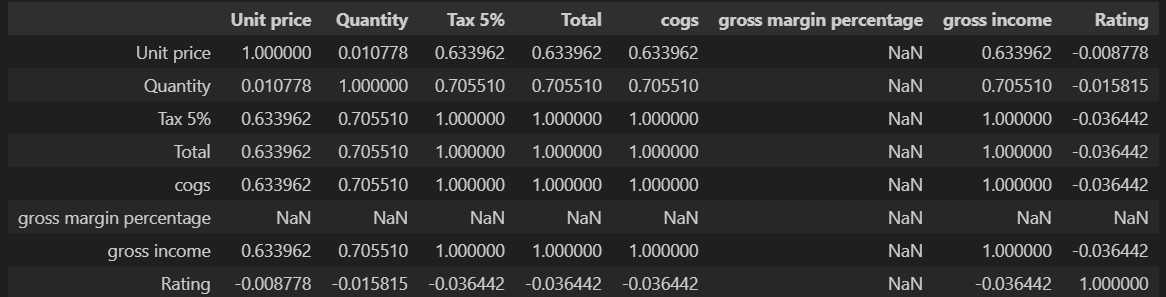
\includegraphics[width=1\textwidth]{Chapters/ch1/ch_1_corr_matrix.png}
    % \caption{This is an example image.}
    % \label{fig:example}
\end{figure}
% \subsection{About this Template}

We can observe a strong positive correlation between Unit Price, Quantity, Tax 5\%, Total, COGS, and Gross Income, suggesting that increases in one tend to correspond with increases in the others. However, the Gross Margin Percentage lacks variability in the given dataset, resulting in undefined correlations with other variables. Rating exhibits a very weak negative correlation with Unit Price, Quantity, Tax 5\%, Total, COGS, and Gross Income, implying that changes in Rating are not strongly associated with changes in these variables.


%----------------------------------------------------------------------------------------


\begin{figure}[h]
    \centering
    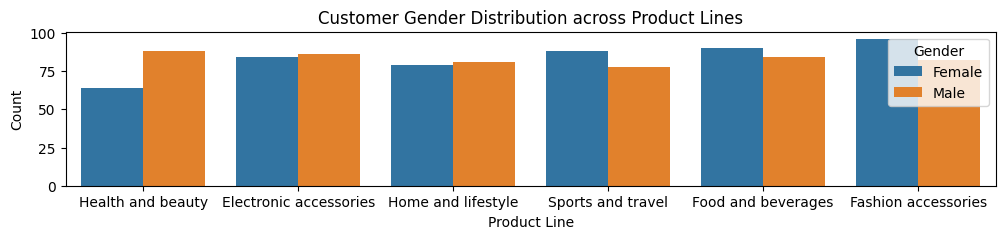
\includegraphics[width=1\textwidth]{Chapters/ch1/ch_1_barchart_1.png}
    % \caption{This is an example image.}
    % \label{fig:example}
\end{figure}
% \subsection{About this Template}

This helps understand how the purchase behavior varies between male and female customers for each product line. For example, it can reveal whether certain product lines are more popular among one gender, providing insights into potential marketing strategies or product positioning. If there's a significant gender bias in product preferences, the business can tailor its offerings accordingly.



%----------------------------------------------------------------------------------------


\begin{figure}[h]
    \centering
    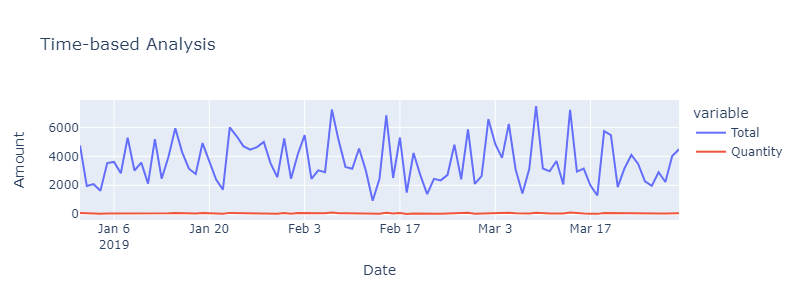
\includegraphics[width=1\textwidth]{Chapters/ch1/ch_1_timeseries_1.png}
    % \caption{This is an example image.}
    % \label{fig:example}
\end{figure}
% \subsection{About this Template}
The line plot shows the overall trend of total sales and quantity sold over the given time.The sharp dips and spikes indicate the variance of the ‘Total’ feature. And the almost-straight, red line indicates, with its stagnancy, a low variation in the feature ‘Quantity’ throughout the months January to March.


%----------------------------------------------------------------------------------------


\begin{figure}[h]
    \centering
    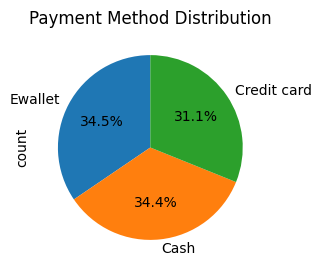
\includegraphics[width=0.5\textwidth]{Chapters/ch1/ch_1_pie_chart_1.png}
    % \caption{This is an example image.}
    % \label{fig:example}
\end{figure}
% \subsection{About this Template}
 This Pie Chart visualization provides insights into the preferred payment methods of customers. Understanding the dominant payment method is crucial for optimizing payment processing systems and ensuring that the most convenient options are available. It also indicates trends in customer preferences and potentially influences decisions related to partnerships with specific payment providers. As can be seen by this chart, all 3 payment modes are near-to-identical and hence preferred almost equally by customers.

%----------------------------------------------------------------------------------------

\begin{figure}[h]
    \centering
    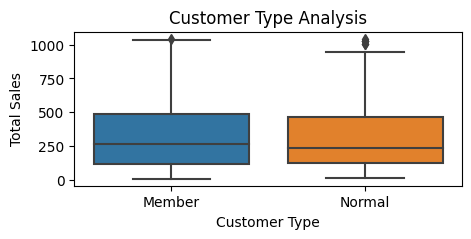
\includegraphics[width=0.8\textwidth]{Chapters/ch1/ch_1_box_plot_1.png}
    % \caption{This is an example image.}
    % \label{fig:example}
\end{figure}
% \subsection{About this Template}

This provides a visual summary of the distribution of total sales for each customer type. There seem to be few outliers beyond the whiskers, indicating high sales for a few examples. Outliers for non-members could indicate specific cases where non-members made exceptionally high purchases.


%----------------------------------------------------------------------------------------

{Exploring the performance of each branch based on total sales and average ratings:}

\begin{figure}[h]
    \centering
    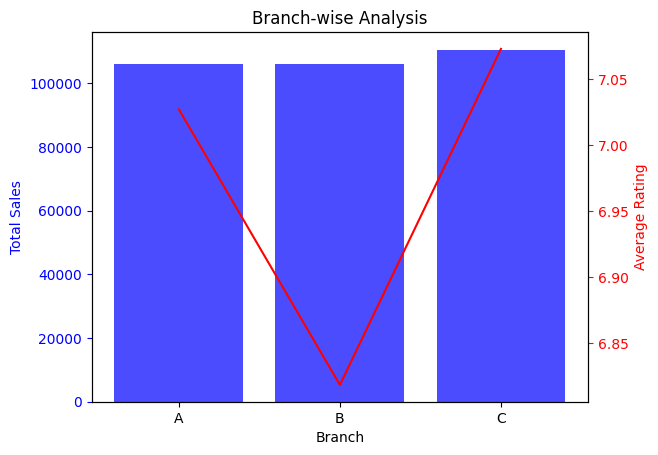
\includegraphics[width=0.5\textwidth]{Chapters/ch1/ch_1_barchart_2.png}
    % \caption{This is an example image.}
    % \label{fig:example}
\end{figure}
% \subsection{About this Template}

The blue bars represent the total sales for each branch. The branches here seem to be almost identical in terms of Sales, with Branch C leading the other by just a bit.
The red line represents the average rating for each branch. This helps evaluate the average customer satisfaction (rating) for each branch. An interesting thing to note is the steep descent of Average Rating for Branch B. This indicates that Branch A has the highest average rating, followed by Branch C. Relatively, Branch B has quite a low average rating.
Grouping by Branch:
\begin{lstlisting}[language=Python, frame=none]
branch_analysis = df.groupby('Branch').agg({'Total': 'sum', 'Rating': 'mean'}).reset_index()
\end{lstlisting}
The code groups the dataset by the 'Branch' column, calculating the total sales and average rating for each branch.

%----------------------------------------------------------------------------------------



\begin{figure}[h]
    \centering
    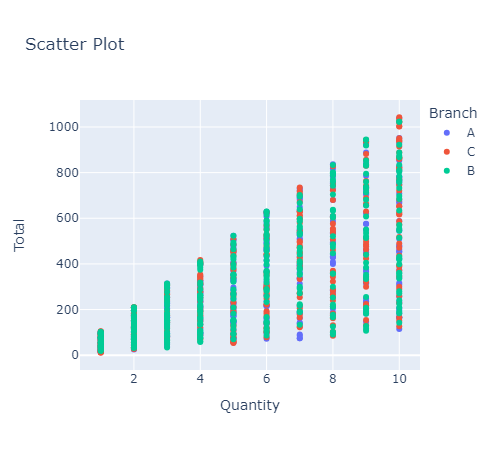
\includegraphics[width=0.5\textwidth]{Chapters/ch1/ch_1_scatter_plot_1.png}
    % \caption{This is an example image.}
    % \label{fig:example}
\end{figure}
% \subsection{About this Template}
This scatter plot represents the relationship between the 'Quantity' and 'Total' columns, with each point corresponding to a specific invoice. The color of the points is differentiated based on the 'Branch' column, and additional information about the 'Product line' is available when hovering over each point in the ipynb file.
This interactive plot allows us to explore the relationship between the quantity and total sales.


